\documentclass[a4paper,10pt]{article}
\usepackage[french]{babel}
\usepackage[utf8]{inputenc}
\usepackage[left=2.5cm,top=2cm,right=2.5cm,nohead,nofoot]{geometry}
\usepackage{url}
\usepackage{graphicx}
\usepackage{float}
\usepackage[colorinlistoftodos]{todonotes}
\usepackage{hyperref}
\usepackage{amssymb}
\usepackage{dsfont}
\usepackage{amsmath}

\linespread{1.1}



\begin{document}

\begin{titlepage}
\begin{center}
\textbf{\textsc{UNIVERSIT\'E DE MONTR\'EAL}}\\
%\textbf{\textsc{Faculté des Sciences}}\\
%\textbf{\textsc{Département d'Informatique}}
\vfill{}\vfill{}
\begin{center}{\Huge Rapport : Devoir2 }\end{center}{\Huge \par}
\begin{center}{\large Pierre Gérard \\ Mathieu Bouchard}\end{center}{\Huge \par}
\vfill{}\vfill{} \vfill{}
\begin{center}{\large \textbf{IFT3395-6390 Fondements de l'apprentissage machine}}\hfill{\\Pascal Vincent, Alexandre de Brébisson et César Laurent}\end{center}{\large\par}
\vfill{}\vfill{}\enlargethispage{3cm}
\textbf{Année académique 2015~-~2016}
\end{center}
\end{titlepage}

%\begin{abstract}
%Ce rapport présente ...
%\end{abstract}


%\tableofcontents

%\pagebreak

\section{Partie théorique: Calcul du gradient pour l’optimisation des paramètres d'un réseau de neurones}

Commençons par dessiner un rapide schéma du réseau de neurones étudié.

\begin{figure}[H]
	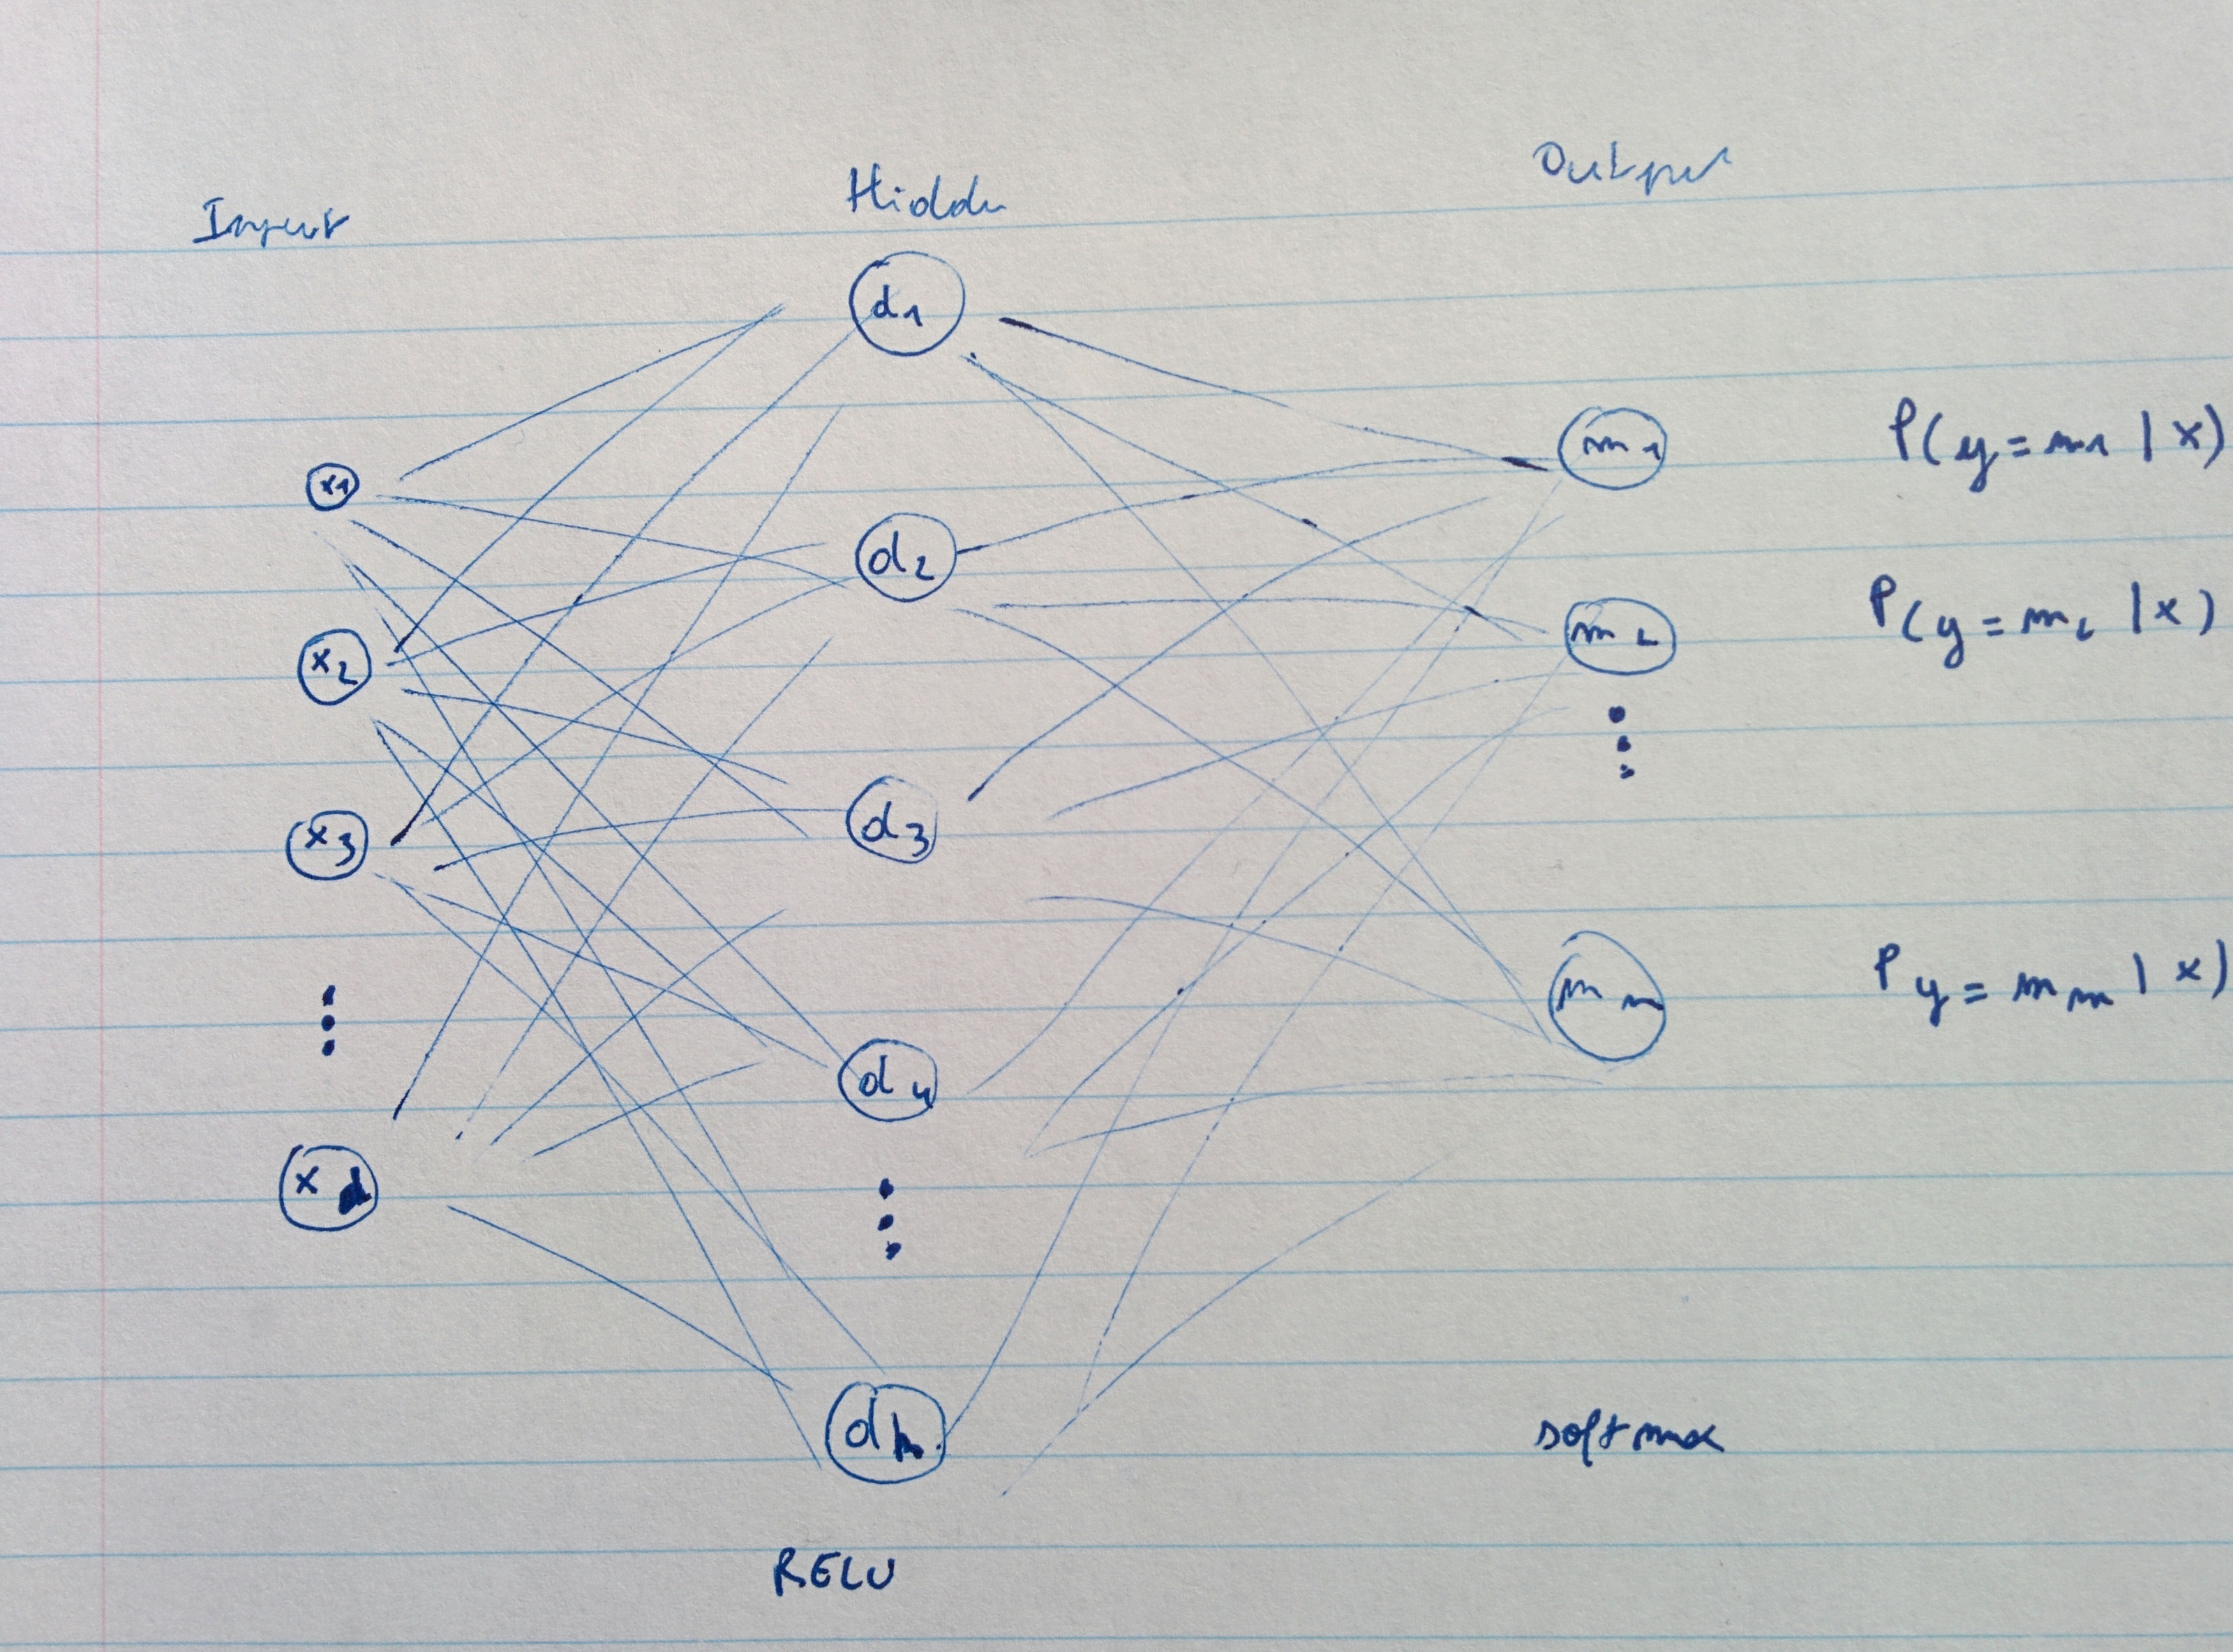
\includegraphics[width=12cm]{reseau.jpg}
	\centering
	\label{fig:comp}
\end{figure}

\subsection{Exercice a)}

b est de dimension $d_{h}$

Le vecteur d'activation est : $h_{a} = W^{(1)}x +b$

Avec $ h_{a_i} = W^{(1)}_{i1} x_{1}  W^{(1)}_{i2} x_{2} + ... + W^{(1)}_{id} x_{d} b_{i}$

Et $h_{s_i} = h_{a_i}*I_{ \{ h_{a_i} > 0 \} } = max(h_{a_i}, 0)$

\subsection{Exercice b)}

$W^{(2)}$ est de dimension $m \times d_{h}$

$b^{(2)}$ est de dimension $m$

Le vecteur d'activation est : $o^{a} = W^{(2)} h_{s} + b^{(2)}$

Avec $o^{a}_{k} = W^{(2)}_{k1} h_{s_1} + W^{(2)}_{k2} h_{s_2} + ... + W^{(2)}_{kn} h_{s_n} + b^{(2)}_{k}$

\subsection{Exercice c)}

$o^{s} = softmax(o^{a}) = \frac{1}{\sum_{i=1}^{m} e^{o^{a}_{i}}}  (e^{o^{a}_{1}}, e^{o^{a}_{2}}, ..., e^{o^{a}_{n}})$

Donc $o^{s}_{k} = \frac{e^{o^{a}_{k}}}{\sum_{i=1}^{m} e^{o^{a}_{i}}}$

$e^{x} : \mathds{R} \rightarrow \mathds{R}^{+}$ donc la somme au numérateur de la fonction ci-dessus sera positive et la somme au numérateur aussi. Une fraction de deux nombres positifs sera toujours positif donc $o^{s}_{k}$ est toujours positif.

$\sum^{m}_{i=1} o^{s}_{i} = \sum^{m}_{i=1} \frac{e^{o^{a}_{i}}}{\sum_{j=1}^{m} e^{o^{a}_{j}}}$

$ = \frac{1}{\sum_{j=1}^{m} e^{o^{a}_{j}}} \sum^{m}_{i=1} e^{o^{a}_{i}}$

$ = \frac{\sum^{m}_{i=1} e^{o^{a}_{i}}}{\sum_{j=1}^{m} e^{o^{a}_{j}}}$

$ =1 $


C'est important car cela signifie que les sorties sont les probabilité pour l'entrée d'être d'une certaine classe et ces classes sont mutuellement exclusives.

\subsection{Exercice d)}

$ L(x,y) = -log  (o^{s}_{y}(x)) $

$= -log \frac{e^{o^{a}_{y}(x)}}{\sum_{i=1}^{m} e^{o^{a}_{i}(x)}}$ 

$= -log(e^{o^{a}_{y}(x)}) +log(\sum_{i=1}^{m} e^{o^{a}_{o}(x)})  $

$ = -o^{a}_{y}(x) + log(\sum_{i=1}^{m} e^{o^{a}_{i}(x)})$

\subsection{Exercice e)} 

L'erreur empirique vaut :

$\widehat{R}(f,D) = \sum_{i=1}^{n} L(x,y)$

\todo{demander en tp des précisions sur la notation ci-dessus}

Les paramètres sont :

$ \theta = \{ W^{(1)},W^{(2)},b^{(1)},b^{(2)} \}$ avec $W^{(1)}$ et $b^{(1)}$ représentant les connexions synaptiques entre l'entrée et la couche cachée et $W^{(2)}$ et $b^{(2)}$ représentant les connexions synaptiques entre la couche cachée et la sortie.

Le problèmes d'optimisation revient donc à l'équation suivante :

$\theta^{*} = argmin_{\theta} \widehat{R}(f,D) $

Les dimensions sont :

$n_{\theta}$ est de dimension $d_{h} \times d + d_{h} + m \times d_{h} + m$

\subsection{Exercice f)} 

\begin{verbatim}
	def gradient(ensemble_donne):
.		somme = 0
.		for x in ensemble_donne:
.		.	sum += derivation_lost(x)
.		return somme
\end{verbatim}

\begin{verbatim}
	theta = initialisation des params de maniere random
	epsilon =
	learningRate =
	while learningRate*gradient() < epsilon :  # attention aux boucles infini
.		theta = theta + learningRate*gradient()
\end{verbatim}
\subsection{Exercice g)}
\todo{Comment ajouter de l'espace entre les lignes pour que ce soit plus lisible?}
Pour $k \neq y$:

$\frac{\partial L}{\partial {O^a_k}} = \frac{\partial}{\partial O^a_k} ( -O^a_y (x)+ log \sum_{i=1}^{m} e^{O^a_i(x)})$

$= 0 + \frac{\partial}{\partial O^a_k} log \sum_{i=1}^{m} e^{O^a_i(x)}$

$= \frac{\frac{\partial}{\partial O^a_k} \sum_{i=1}^{m} e^{O^a_i(x)}}{\sum_{i=1}^{m} e^{O^a_i(x)}}$

$= \frac{\frac{\partial}{\partial O^a_k} e^{O^a_k(x)}}{\sum_{i=1}^{m} e^{O^a_i(x)}}$

$= \frac{e^{O^a_k(x)}}{\sum_{i=1}^{m} e^{O^a_i(x)}}$

Pour $k=y$:

$\frac{\partial L}{\partial {O^a_y}} = \frac{\partial}{\partial O^a_y} ( -O^a_y (x)+ log \sum_{i=1}^{m} e^{O^a_i(x)})$

$= \frac{-\partial O^a_y}{\partial O^a_y} + \frac{\partial}{\partial O^a_y} log \sum_{i=1}^{m} e^{O^a_i(x)}$

$= -1+\frac{e^{O^a_y(x)}}{\sum_{i=1}^{m} e^{O^a_i(x)}}$

Le premier terme du résultat vaut donc $-1$ seulement lorsque $k=y$ et 0 sinon. On obtient alors:

$\frac{\partial L}{\partial {O^a_k}} = \frac{1}{\sum_{i=1}^{m} e^{O^a_i(x)}} (e^{O^a_1(x), e^{O^a_2(x)}, ..., e^{O^a_m(x)}}- onehot_m(y)) = O^s - onehot_m(y)$

\subsection{Exercice h)}


\begin{verbatim}
	import numpy as np
	grad_oa = 1/np.sum(e_oa) * np.array(e_oa)   # avec e_oa correspondant à np.exp(oa)
	grad_oa[y] = grad_oa[y] - 1  #onehot
\end{verbatim}

\subsection{Exercice i)}
Réponse entière donnée

\subsection{Exercice j)} 

La dimension de :
\begin{itemize}
	\item $\frac{\partial L}{\partial b^{(2)}}$ est $m$
	\item $\frac{\partial L}{\partial W^{(2)}}$ est $ m \times d_{h}$
	\item $\frac{\partial L}{\partial o^{a}}$ est $ m \times 1$
	\item $h^{s^T}$ est $ 1 \times d_{h}$
\end{itemize}

\begin{verbatim}
	grad_b2 = grad_oa
	grad_w2 = grad_oa * np.transpose(h_s)
\end{verbatim}

\subsection{Exercice k)}
Réponse entière donnée

\subsection{Exercice l)}

La dimension de :
\begin{itemize}
	\item $\frac{\partial L}{\partial h^{s}}$ est $d_{h}$
	\item $W^{(2)^T} $ est $d_{h} \times m$
	\item $\frac{\partial L}{\partial o^{a}}$ est $ m \times 1$
\end{itemize}

\begin{verbatim}
 grad_hs = np.transpose(w_2) * grad_oa	
\end{verbatim}

\subsection{Exercice m)}

\todo{formatter acollade}

$\frac{\partial rect(z)}{\partial z} = \frac{\partial max(0,z)}{\partial z} = \lbrace {0 si z \leq 0 \\ 1 sinon}$

Pour $h^a_j \leq 0$:

$\frac{\partial L}{\partial h^a_j} = \frac{\partial L}{\partial h^s_j} \frac{\partial h^s_j}{\partial h^a_j} = \frac{\partial L}{\partial h^s_j} \frac{\partial rect(h^a_j)}{\partial h^a_j} = \frac{\partial L}{\partial h^s_j}*0 = 0$

Pour $h^a_j > 0$:

$\frac{\partial L}{\partial h^a_j} = \frac{\partial L}{\partial h^s_j} \frac{\partial h^s_j}{\partial h^a_j} = \frac{\partial L}{\partial h^s_j} \frac{\partial rect(h^a_j)}{\partial h^a_j} = \frac{\partial L}{\partial h^s_j}*1 = \frac{\partial L}{\partial h^s_j}$

Au final:
\todo{formatter acollade}

$\frac{\partial L}{\partial h^a_j} = \lbrace 0 si h^a_j \leq 0 \frac{\partial L}{\partial h^s_j} sinon$

$\frac{\partial L}{\partial h^a_j} = \frac{\partial L}{\partial h^s_j} * I_{\lbrace h^a_j > 0 \rbrace} $

\subsection{Exercice n)}

\todo{Possible de simplifier l'expression de ce vecteur?}
$\frac{\partial L}{\partial h^a} = \begin{bmatrix}
		\frac{\partial L}{\partial h^s_1} * I_{\lbrace h^a_1 > 0 \rbrace} \\
		\frac{\partial L}{\partial h^s_2} * I_{\lbrace h^a_2 > 0 \rbrace}\\
		\vdots \\
		\frac{\partial L}{\partial h^s_{d_h}}* I_{\lbrace h^a_{d_h} > 0 \rbrace}
		\end{bmatrix}$ qui est une vecteur colonne de taill $d_h$



\begin{verbatim}
	grad_ha = (grad_hs + np.abs(grad_hs))/2  # astuce pour garder que les nombre positif
\end{verbatim}


\subsection{Exercice o)}

Pour $b^{(1)}$ :

$\frac{\partial L}{\partial b^{(1)}_{k}} = \frac{\partial L}{\partial h^{a}_{k}} \frac{\partial h^{a}_{k}}{\partial b^{(1)}_{k}}$

$ = \frac{\partial L}{\partial h^{a}_{k}} \frac{\partial \sum_{j'} W^{(1)}_{kj'} x_{j} + b^{(1)}_{k}}{\partial b^{1}_{k}}$

$ = \frac{\partial L}{\partial h^{a}_{k}}$

Pour $W^{(1)}$ :

$\frac{\partial L}{\partial W^{(1)}_{kj}} = \frac{\partial L}{\partial h^{a}_{k}} \frac{\partial h^{a}_{k}}{\partial W^{(1)}_{kj}} $

$ = \frac{\partial L}{\partial h^{a}_{k}} \frac{\partial \sum_{j'} W^{(1)}_{kj'} x_{j} + b^{(1)}_{k}}{\partial W^{(1)}_{kj}}$

$ = \frac{\partial L}{\partial h^{a}_{k}} x_{j} $


\subsection{Exercice p)}

Expressions matricielles:

$\frac{\partial L}{\partial b^{(1)}} = \frac{\partial L}{\partial h^a}$

$\frac{\partial L}{\partial W^{(1)}} = \frac{\partial L}{\partial h^a}(x)^T$

La dimension de :
\begin{itemize}
	\item $\frac{\partial L}{\partial b^{1}}$ est $d_{h}$
	\item $\frac{\partial L}{\partial W^{(1)}}$ est $d_{h} \times n$ car  $\frac{\partial L}{\partial h^{(a)}}$ est $d_{h} \times 1$ et $ x $ est $1 \times n$
\end{itemize}

\begin{verbatim}
	grad_b1 = grad_ha
	grad_w1 = grad_ha * np.transpose(x)
\end{verbatim}


\subsection{Exercice q)}

$\frac{\partial L}{\partial x_j} = \sum_{k=1}^{n} \frac{\partial L}{\partial h_k^a} \frac{\partial h_a^k}{\partial x_j}$

$ = \sum_{k=1}^{n} \frac{\partial L}{\partial h_k^a} (\frac{\partial }{\partial x_j} \sum_{j'} W^{(1)}_{kj'} x_{j'} + b^{(1)}_k$

$ = \sum_{k=1}^{n} \frac{\partial L}{\partial h_k^a} W^{(1)}_{kj} x_{j}$

Sous forme matricielle, on obtient:

$\frac{\partial L}{\partial x} = {W^{(1)}}^T \frac{\partial L}{\partial h^a}$

\todo{validation: ca semble correcte}


\subsection{Exercice r)}

\end{document}
